\documentclass{aastex6}
\usepackage{graphicx}
\usepackage{float}
\usepackage{subfigure}
\graphicspath{{/home/rafia/Desktop/Paper/}}


\begin{document}

\title{Analyzing NIRCam Test Data}
\author{Rafia Bushra, Everett Schlawin and Jonathan Fraine}
\affil{Department of Astronomy/Steward Observatory\\
University of Arizona}



\begin{abstract}
The James Webb Space Telescope (JWST) is a near- and mid-infrared optimized space telescope. It will have unprecedented sensitivity and will be able to see objects fainter and further than those detectable by previous telescopes like the Hubble Space Telescope (HST). Thus, JWST will have tremendous applications in the field of exoplanets. The telescope is equipped with four sensitive instruments: NIRCam, MIRI, NIRSpec and NIRISS that will cover a wavelength range of 0.6 - 28 microns. Of these instruments, NIRCam will be the primary imager in 0.6 - 5 microns and perform spectroscopy in 2.4 - 5.0 microns wavelength ranges . At NASA Goddard’s cryogenic vacuum facility in Greenbelt, Maryland, The NIRCam instrument module was used to take extensive images in a controlled environment over several months. The data gathered in the tests is the subject of this article. The images obtained from these tests were used to create light curves to simulate  real observations of exoplanets with JWST. This article deals with the extraction process of the time series data and examining different analysis techniques to determine what works best for processing the data as interest grows in pushing JWST to new limits to observe Earth-like planets such as TRAPPIST-1d or LHS 1140 b.
\end{abstract}



\section{Introduction}
The JWST will revolutionize the field of exoplanetary sciences. The telescope's sensitivity combined with the broad range of wavelength coverage (0.6 - 28 microns) enables it to make accurate measurement of transits. JWST will also look in planetary atmospheres to determine chemical composition and evolution. Most planets however, are quite small compared to their host stars and their atmospheres are even smaller. Thus, understanding atomic and molecular composition in transiting exoplanets requires very precise measurements at precision levels of around 30 parts per million. To achieve that kind of sensitivity, we will need to understand every detail of the telescope, camera and electronics.\\
To understand the details of the telescope and it's camera, the instrument modules have been used to run simulations and gather data. The collected data is converted to fits files, which we will use to extract time series and create light curves. In this paper, we will be describing the steps we took to extract the data, to increase the accuracy of measurements and discuss the methods that worked best in analyzing the data.   



\section{Procedure}
As mentioned above, this paper deals with analyzing NIRCam test data to extract time series and create light curves. Light curve is a plot demonstrating the variation of light received from a source over a certain amount of time. For the test, electrical lamps were used as light source.\\
The first step in creating a light curve is extracting flux and the corresponding time intervals. However, there are some complications in that process e.g. generating separate centers for each image, deciding on an aperture radius, subtracting background noise etc. \\
Unless otherwise mentioned, flux comparison in all tests uses background subtracted, averaged(over A \& B detector) flux; For all tests, standard deviation is measured after detrending the data with a linear best fit. To properly describe the whole method, we have divided it into small sections and briefly described them below.   


    \subsection{Extracting Flux and Time}
    This is the first step of creating a light curve.\\
    The time for each image in a test is extracted from some information provided in the header of the fits file. Time is calculated using the following formula:
    $$Time =  (NGROUP  + 1) * TGROUP * (ON\_NINT - 1)$$ 
    Where, \\
    $NGROUP$ = Number groups in an integration\\
    $TGROUP$ = Delta time between groups\\
    $ON\_NINT$ = INT of total number of NINT in original file\\
    These are information that can be found in the header of the respective fits file. \\
    Extracting flux involves many small components and thus deserves to be broken down to subdivisions. So the next few subsections will sequentially describe how we extracted the Flux.

        \subsubsection{Generating Slope Images}
        Flux is calculated in data numbers per second ($DN/s$), so it is a slope calculated from the data. There are different ways to generate slope images.\\
        If the files are in .slp format, they can be used as is because the slopes have already been calculated. The .slp files should be used if $NGROUP > 2$ because then there is enough reads for a good fit.\\
        If $NGROUP = 2$, the .red formats should be used. The slopes are not calculated and there are 2 reads to calculate the slope from. There are two ways to calculate the slope.\\
        The first is called the Slope1 method, also known as CDS (Correlated Double Subtraction). In this method, slope is calculated using the following formula:
        $$\frac{(Last Group - First Group)}{(NGROUP-1)*TGROUP}$$
        The second method for calculating slope from a .red file is the Slope2 method. Slope is calculated in the following way:
        $$\frac{(Last Group - Bias)}{NGROUP*TGROUP}$$
        After comparison, we found that the Slope2 method gives better results. This is demonstrated in the figure below.
        \begin{figure}[H]
            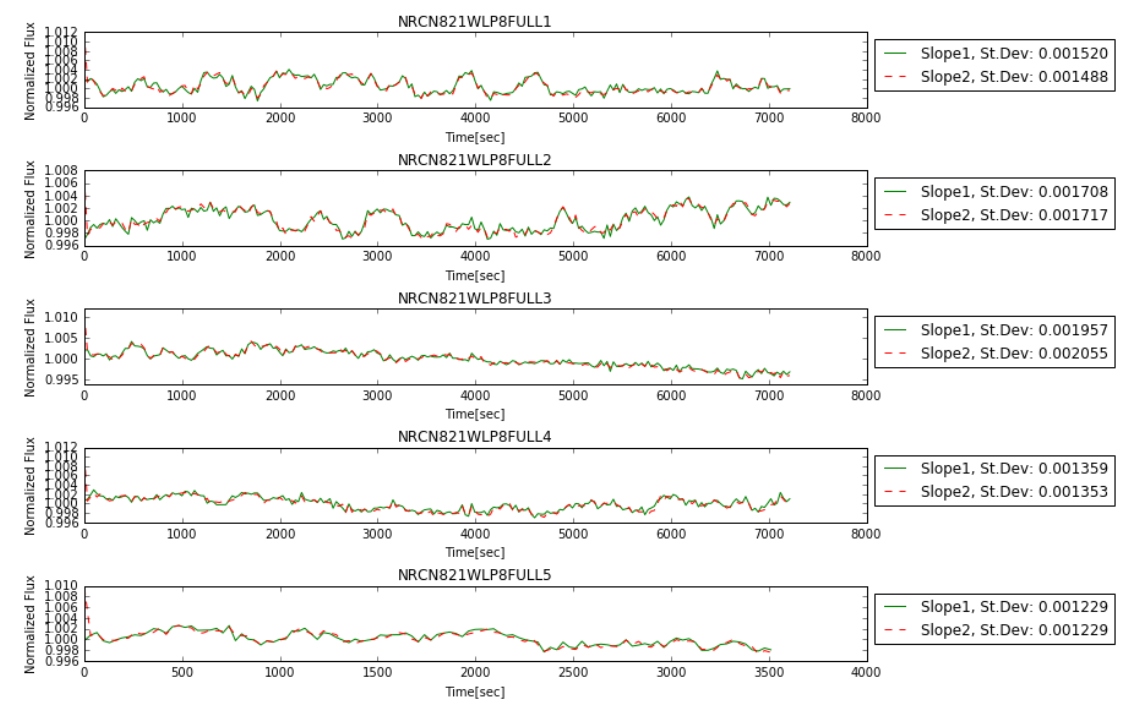
\includegraphics[width=1.0\textwidth]{Slopes}
            \caption{Plot demonstrating light curves \& standard deviations obtained using Slope1 and Slope2 methods for 5 different tests.}
            \label{fig:slopes}
        \end{figure}
        So wherever applicable, we will be using the Slope2 method.   
        
        \subsubsection{Generating Centers}
        For the same test, for a particular detector, expecting all the images to share a common center is a good approximation but not very accurate. The center position is slightly for each image in the time series. This is demonstrated below:
        
        \begin{figure}[H]
            \begin{centering}
            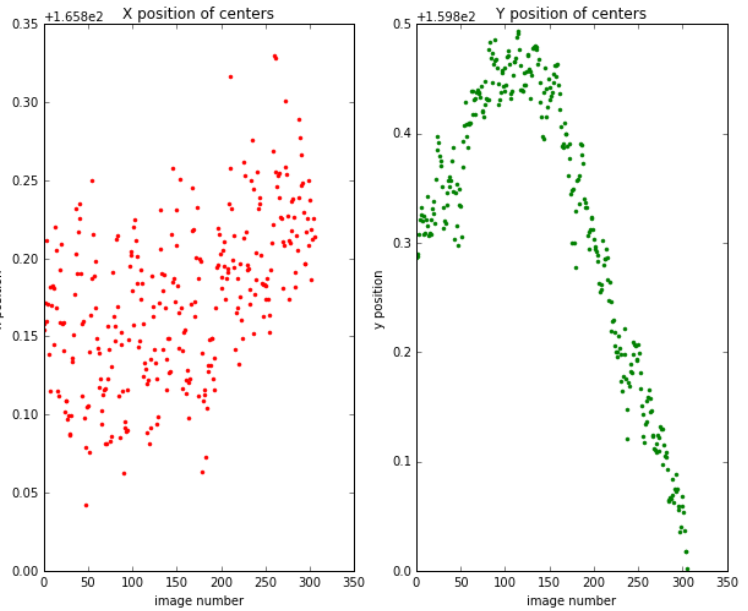
\includegraphics[width=0.5\textwidth]{center_positions}
            \caption{Center positions Vs. image number. The x-axis represents each individual image in the time series}
            \end{centering}
        \end{figure}
        
        So we need speratecenter positions for each individual image. If the model's center is fitted to a Gaussian model, that gives a much closer approximation of an individual image's center. Here is an example Gaussian fit:
        
        \begin{figure}[H]
            \begin{centering}
                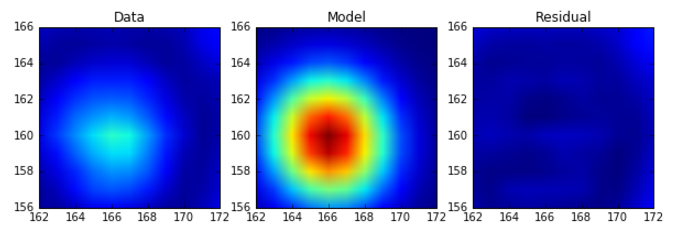
\includegraphics[scale=0.5]{Gaussian}
                \caption{Example of Gaussian fitting to an image's center}
            \end{centering}
        \end{figure}
        The flux is extracted using circular aperture, for which the center is needed. When extracting flux from each image of a test, their individual center obtained from Gaussian fitting will be used.  
        
        \subsubsection{Radius Testing}
        The circular aperture function used for flux extraction also requires a radius. This radius is the source radius. The radius has to be chosen so that the measured error or standard deviation is minimum. For this, we extract the flux multiple times using varying radius values and calculate standard deviations. Here is plot showing how the best radius is chosen:
        \begin{figure}[H]
            \begin{centering}
            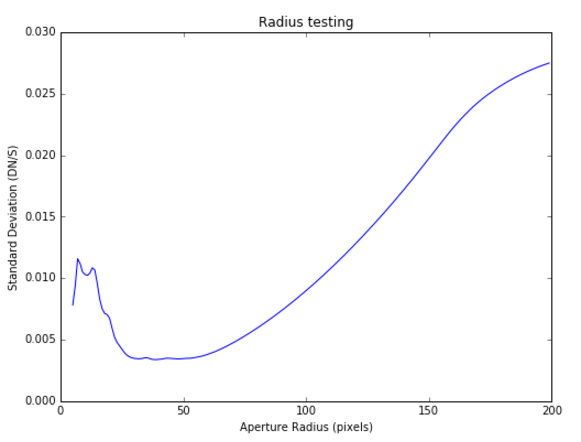
\includegraphics[scale=0.5]{Radius}
            \caption{A plot of Standard Deviation Vs. Aperture Radius. The minimum of the curve gives the best aperture radius}
            \end{centering}
        \end{figure}
        
        Here is a figure to help visualize how much flux is enclosed by different radii:
        
        \begin{figure}[H]
            \begin{centering}
            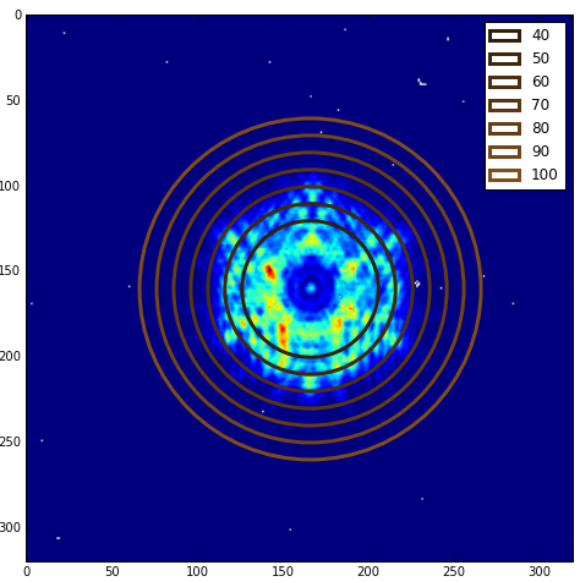
\includegraphics[width=0.5\textwidth]{varying_r.png}
            \caption{Rings of varying radius over the PSF}
            \end{centering}
        \end{figure}
        
        
        \subsubsection{Subtracting Background}
        Other than the light received from the source, there is usually some background noise that we have to account for in order to get more accurate results. For this we are using an annulus out side the source to subtract. For Background subtraction there a few different factors to consider,e.g. the shape of annulus, the type of average, pixel count at the edge of annulus etc. We tested different methods which are a combination of two annulus shapes (circular annulus \& circle inside square (CIS)) and three different types of average (mean, median and MAD(robust average)). We compared our results with circular annulus of astropy which considers fractional pixels at the edge. \\
        
        The annulus has an inner radius and an outer radius. So now, there are three different radii to consider: source radius, inner radius (BG subtraction) and outer radius (BG subtraction). The best combination of these three is determined through a radius test. \\
        
        \begin{figure}[H]
            \centering
            \begin{subfigure}{1}
                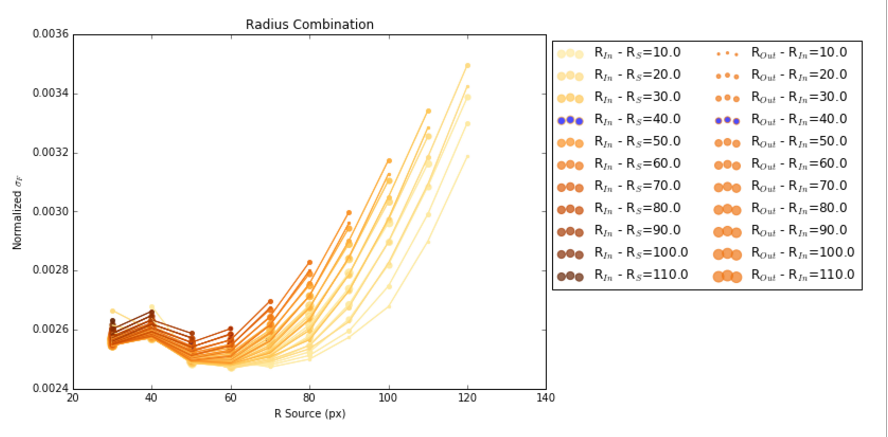
\includegraphics[width = 0.4\textwidth]{Combo}
                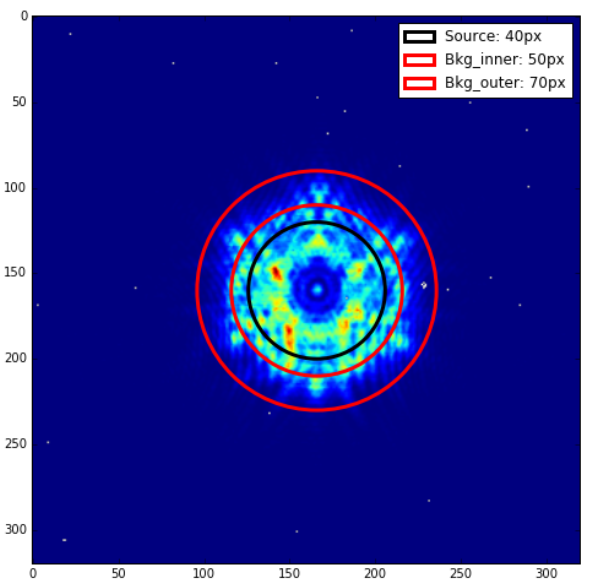
\includegraphics[width = 0.4\textwidth]{sub320_rings}
                \caption{SUB320}
            \end{subfigure}
        
            \begin{subfigure}{2}
                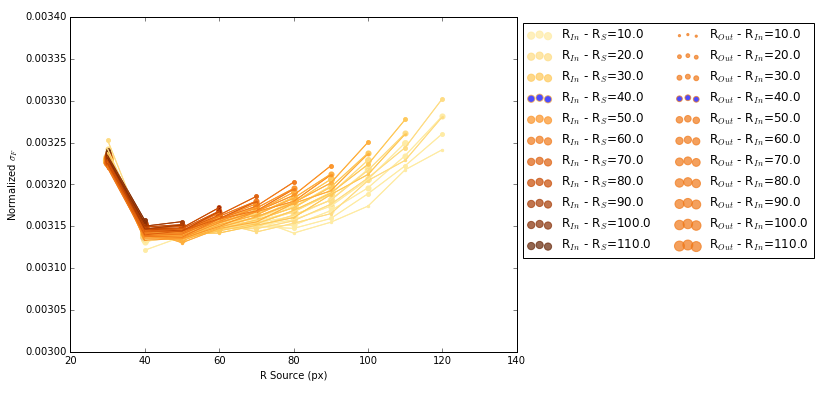
\includegraphics[width = 0.4\textwidth]{Radius_640}
                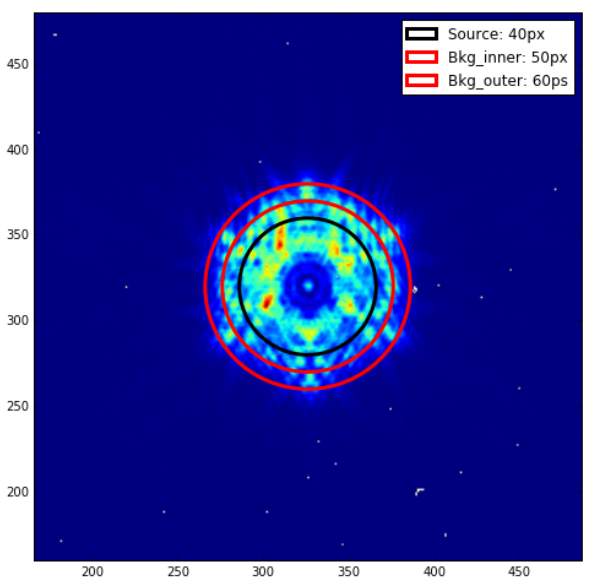
\includegraphics[width = 0.4\textwidth]{sub640_rings}
                \caption{SUB640}
            \end{subfigure}
            
            \begin{subfigure}{3}
                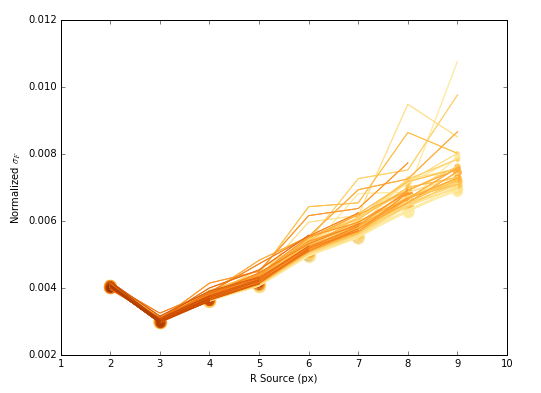
\includegraphics[width = 0.4\textwidth]{Radius_CLR}
                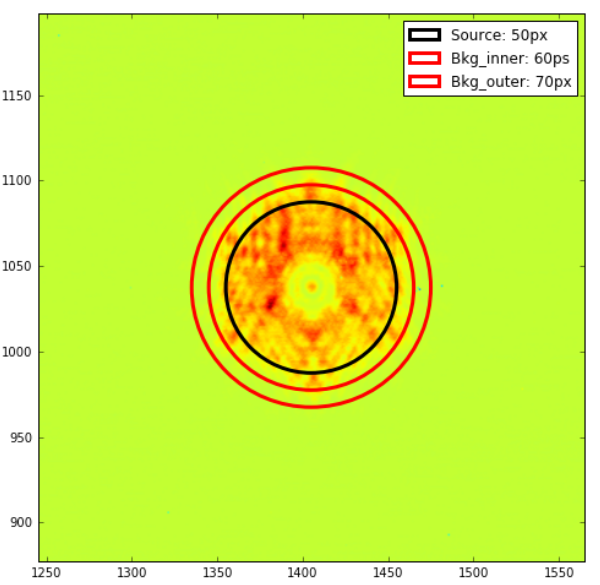
\includegraphics[width = 0.4\textwidth]{full1_rings}
                \caption{CLRSUB}
            \end{subfigure}
            \caption{A plot of Standard Deviation Vs. Source Radius for different combinations of inner and out radii. The minimum of the curves give the best combination}
        \end{figure}
        
        We have also considered two other methods that does not have a particular shape rather is done column by column or row by row. In this method, we considered the background in a single column (or row) at a time, masked source pixels and pixels outside the background range and fit a suitable polynomial to it. We subtracted off the background value of that column from the original one, repeated the process for every column and found the standard deviation of the net residual. For a single column:\\
        
        \begin{figure}[H]
            \centering
            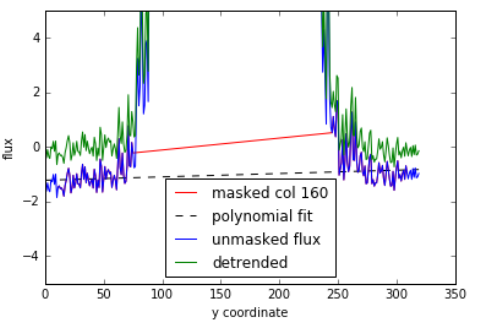
\includegraphics[width = 0.5\textwidth]{col_plot}
            \caption{A plot of the 160th column of an image in its original, masked, fitted and background subtracted versions}
            \end{figure}
            
        Here, the masked points are the background points in the column that remained after masking the source points. As expected, they coincide with the unmasked (original) flux only towards the sides. The detrended curve is what we get after subtracting the polynomial fit to masked points from the original unmasked flux.
        
        Here is a summary of all the methods we used:
        
        \begin{figure}[H]
            \begin{centering}
            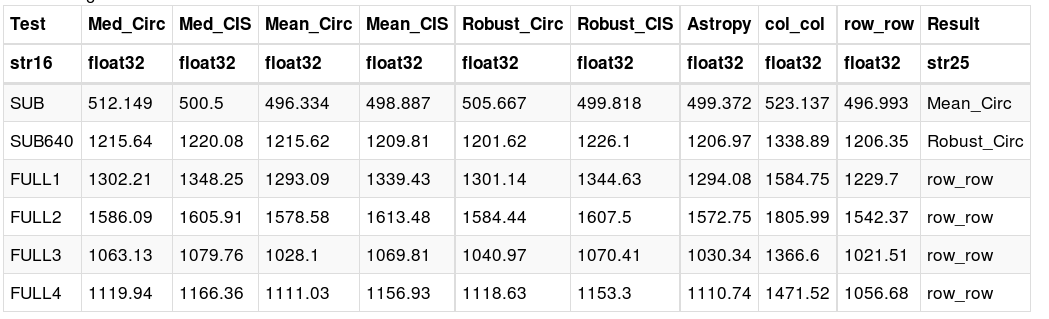
\includegraphics[width=1.0\textwidth]{bkg_sub}
            \caption{Different background subtraction methods. The row by row method works best for the full array tests consistently.}
            \end{centering}
        \end{figure}
        
        The row by row subtracting method makes a significant differece for the full array tests. For the sub array tests, some circular annulus is doing slightly better than row by row and astropy but only by a few parts per million. Since the difference is really small for sub arrays, Astropy might be a better option as it accounts for fractional pixels.\\
        
        
        
        
        \subsubsection{Source Aperture Geometry}
        So far, we kept a basic source aperture (circular aperture) and carried on with other tests like radius combination, gaussian fitting, background subtraction etc. Now that we have a grasp on the other features, we test which source aperture geometry works best with those features. Apart from the circular aperture, we used an annular aperture. \\
        
        \begin{figure}[H]
            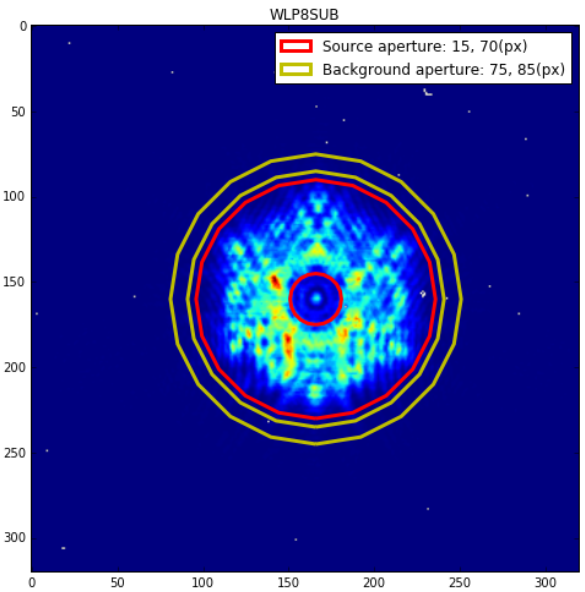
\includegraphics[scale=0.4]{Annular_source}
            \caption{The annular source aperture. Since the center is not as bright as rest of the psf, we picked an annular aperture that envelopes brightest pixels of the psf.}
        \end{figure}
        
        
        \begin{figure}[H]
            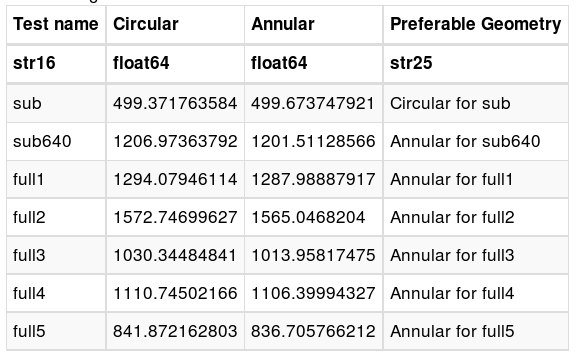
\includegraphics[scale=0.4]{src_ap}
            \caption{Comparing circular and annular source apertures.}
        \end{figure}
        
        The annular aperture, which ignore the relatively dim center gives better results in most cases. It only does worse for WLP8SUB but only ~0.3 ppm.
     
 
    \subsection{Fitting Data To A 1D-Linear Model}
    In order to get the proper standard deviation, the data is fit to a linear model to remove any trend. The data is then divided by the line to get a "de-trended" time series. Here is an example of a linear best fit:
    \begin{figure}[H]
        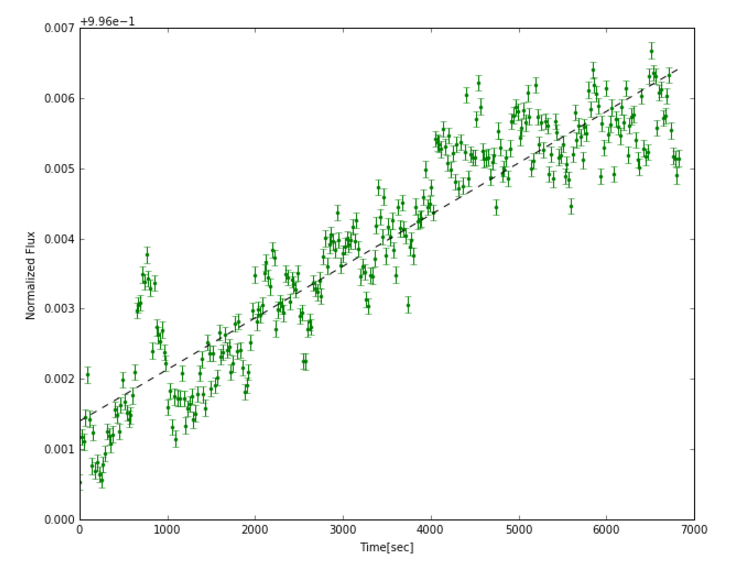
\includegraphics[scale=0.4]{Line}
        \caption{An example linear best fit.}
    \end{figure} 
    
    
    \subsection{Calculating Ideal Noise and Measured Noise}
    The final step in analyzing any test data is calculating the ideal noise and measured noise. Ideal noise is calculated by $$\sigma_F = \frac{\sqrt{Flux*Time*Gain}}{Time*Gain}$$
    The measured noise is the standard deviation of the data. The measured noise (standard deviation) is plotted with time to get a better view of the data. here is an example plot:
    \begin{figure}[H]
        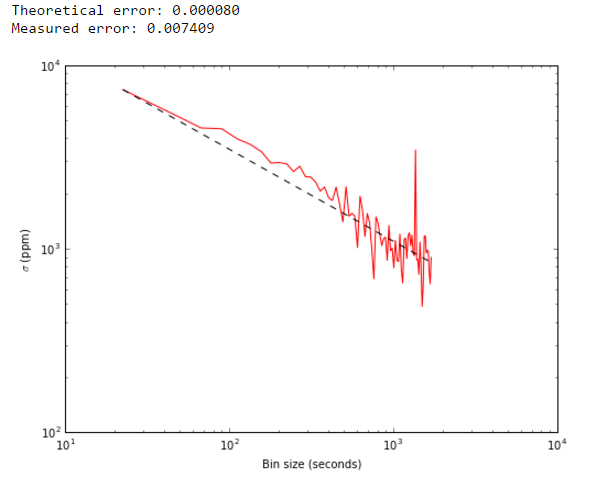
\includegraphics[scale=0.55]{RMS}
        \caption{RMS Vs. Time plot to visualize measured noise}
    \end{figure}



\section{Correction Methods}
There are 3 different correction methods applied to each test: Inter pixel capacitance(IPC) correction, Linearity correction and Flat Fielding. Their combination is denoted with 3 letters (either M(minus, not applied) or P(plus), applied). We tested a few tests to see which combination gives minimum standard deviation and found that the MMM (i.e. no correction method was applied) tests gave the best results. For comparison between different tests, the same radius combination [$(r_{source}, r_{in}, r_{out}) = (70, 72, 80)$] was used for all tests. Here is the result we found:  \\
\begin{figure}[H]
    \centering
    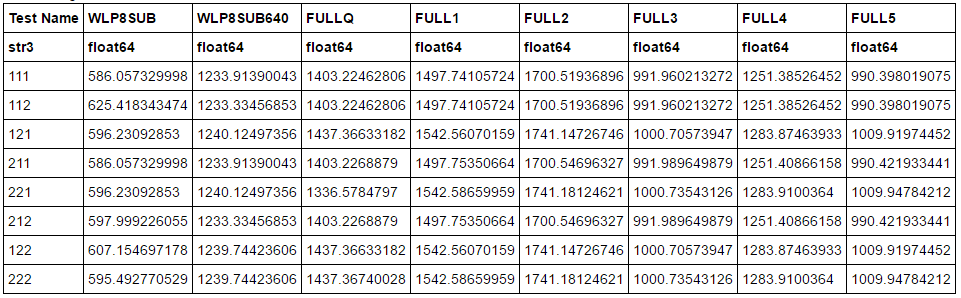
\includegraphics[width=0.7\textwidth]{correction}
    \caption{Table showing the standard deviations for different tests. In the test name column, '1' stands for 'M' and '2' stands for 'P'. E.g. '121' is equivalent to 'MPM'}
\end{figure}
\begin{figure}
    \centering
    \begin{subfigure}{1}
        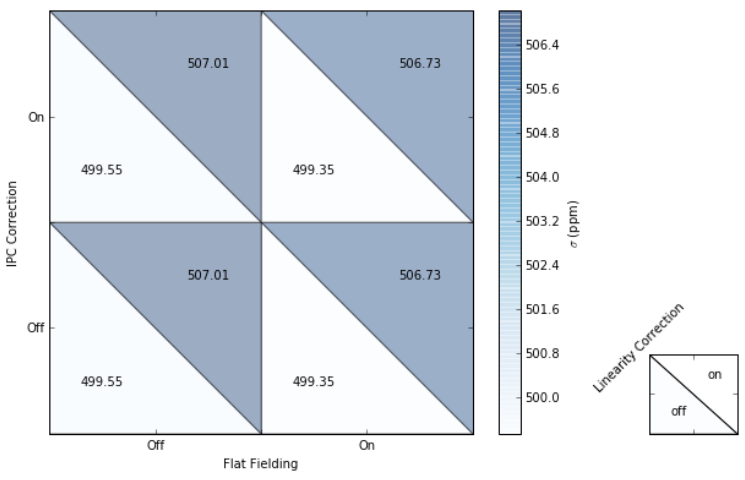
\includegraphics[width=0.45\textwidth]{correction1}
        \caption{Test: WLP8SUB}
    \end{subfigure}
    \begin{subfigure}{2}
        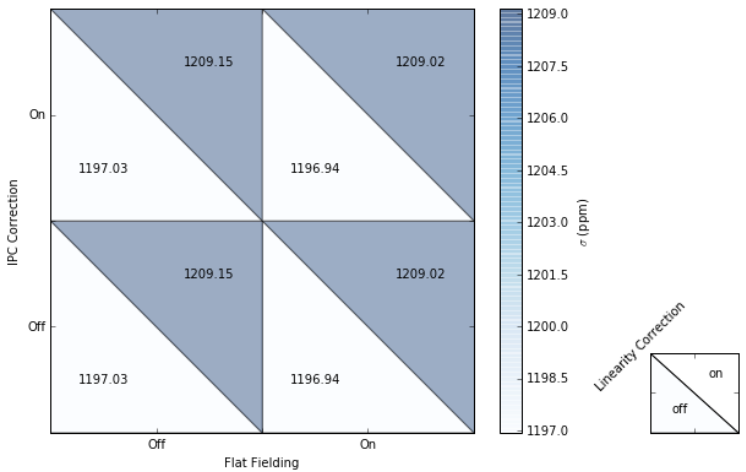
\includegraphics[width=0.45\textwidth]{correction2}
        \caption{Test: WLP8SUB640}
    \end{subfigure}
    \begin{subfigure}{3}
        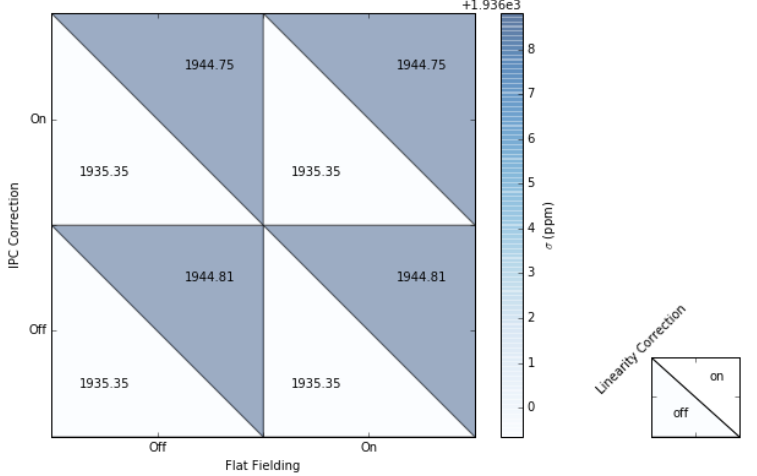
\includegraphics[width=0.45\textwidth]{correction3}
        \caption{Test: FULL1}
    \end{subfigure}
    \caption{A plot showing how standard deviation vary with correction method combinations}
\end{figure}


\begin{figure}[H]
    \centering
    \begin{subfigure}{1}
        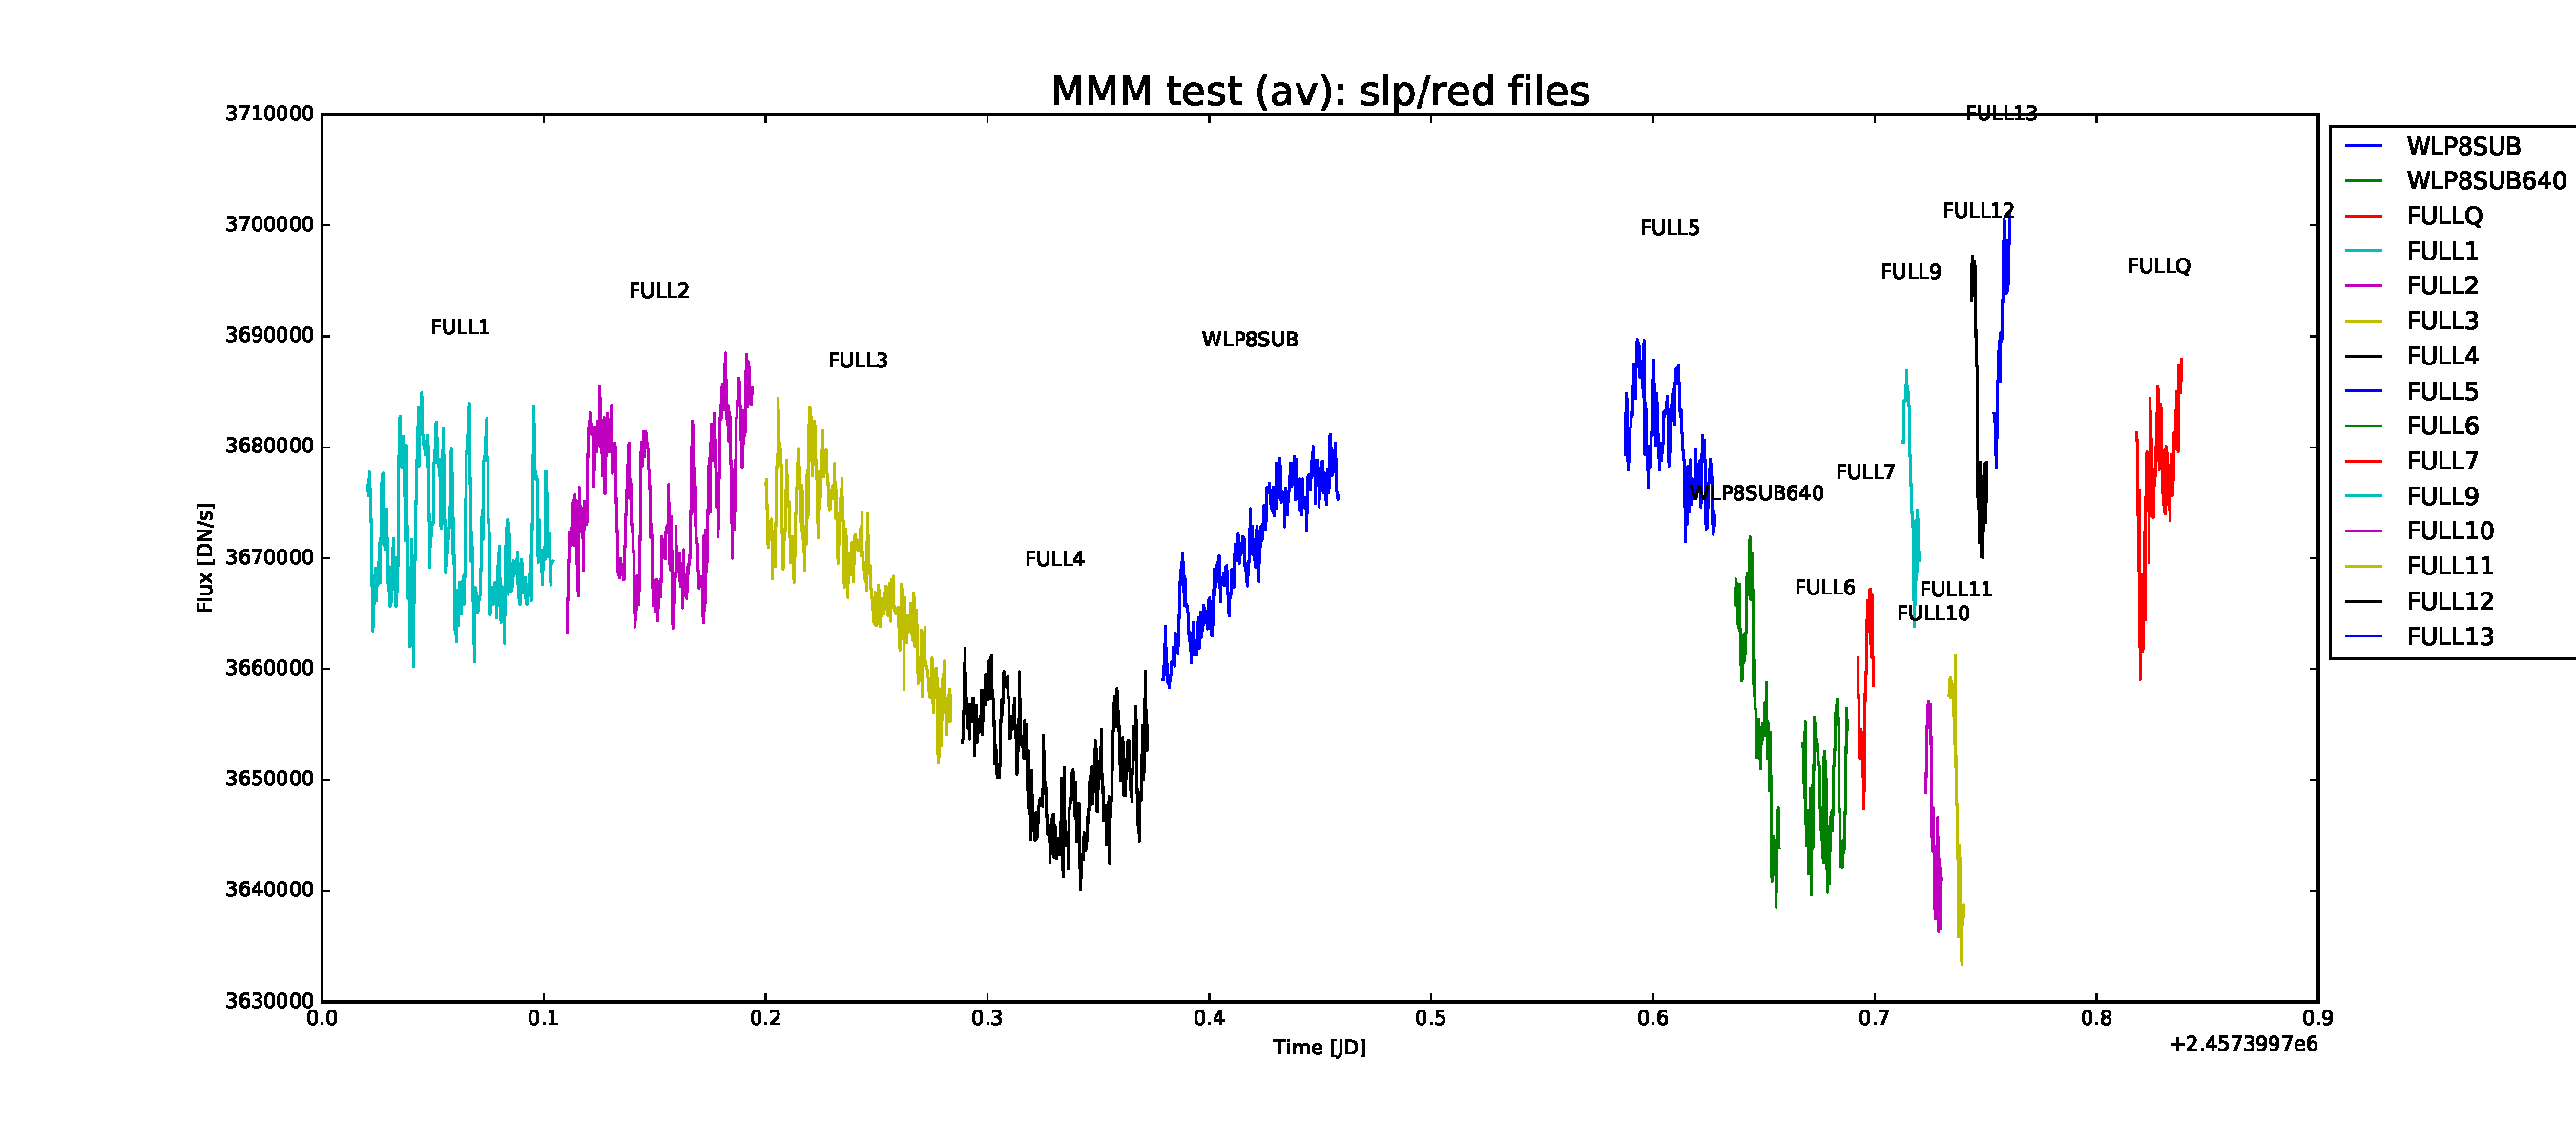
\includegraphics[scale = 0.3]{plot_mmm}
        \caption{MMM}
    \end{subfigure}

    \begin{subfigure}{2}
        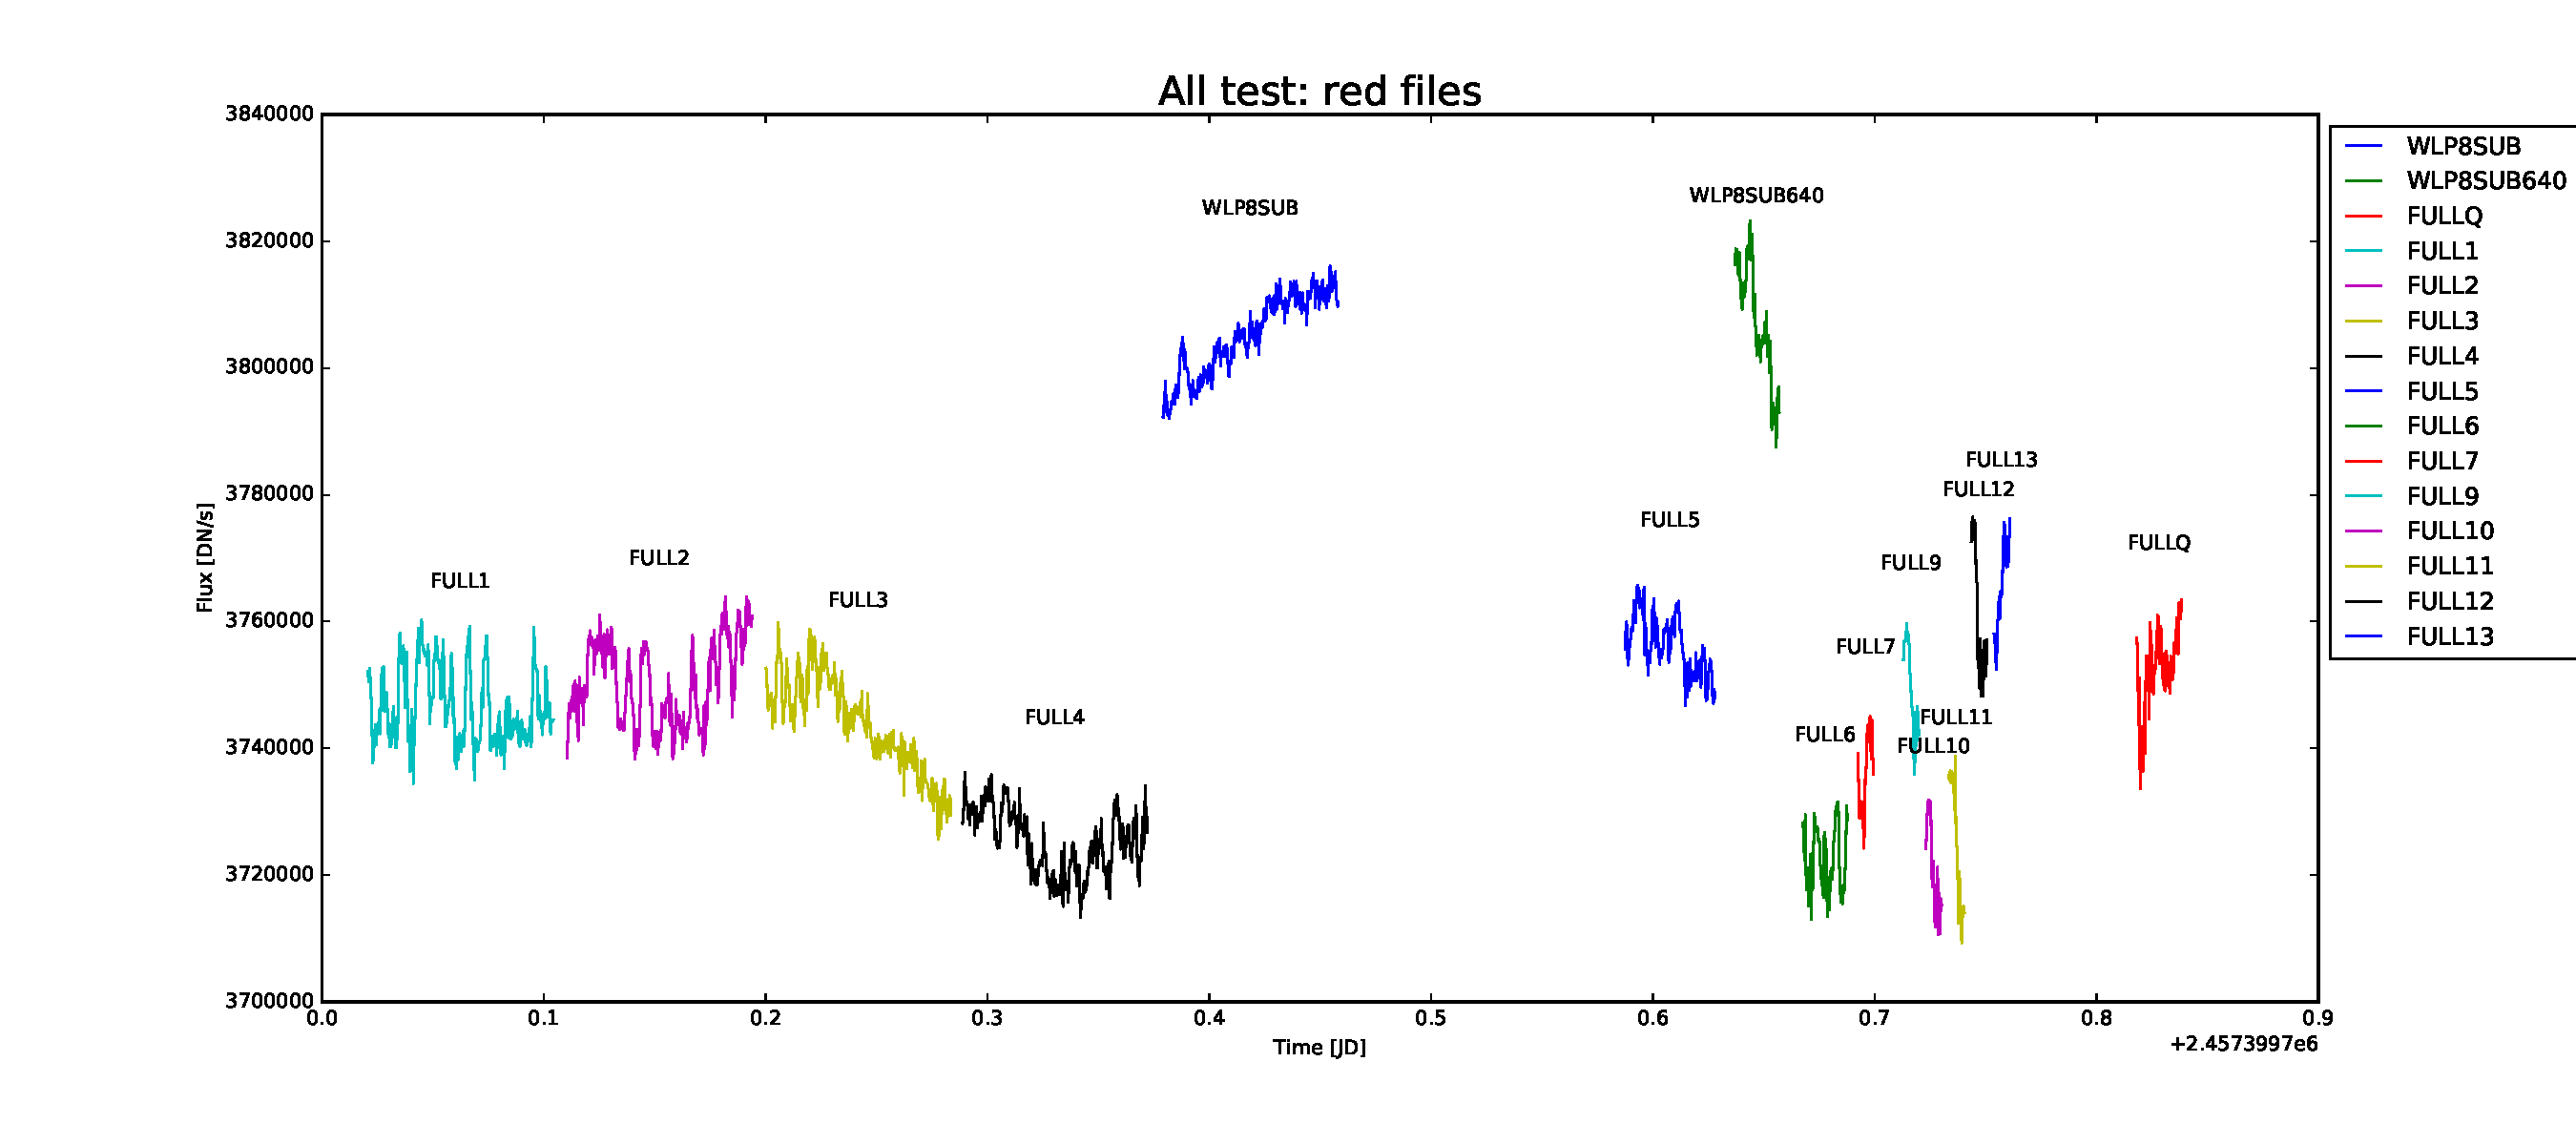
\includegraphics[scale=0.3]{plot_PPP}
        \caption{PPP}
    \end{subfigure}
\end{figure}

As fig. 10. demonstrates, the IPC correction does not make an impact. Linearity correction makes a small difference of about 8ppm and flat fielding has an even smaller effect (a difference of about 0.25ppm). So the correction methods don't play a huge role.  \\




\section{Source Stability}

Since the center position moves around during the tests, we did a test to see how stable the source is. We did this by extracting time series using rectangular apertures on either side of the source center. The configuration looks like:\\


\begin{figure}[H]
    \begin{centering}
    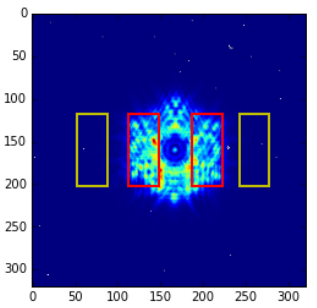
\includegraphics[width=0.5\textwidth]{stability1}
    \caption{Stability test using rectangular apertures.}
    \end{centering}
\end{figure}

The red rectangles are source apertures and yellow ones are background apertures. Two time series can be extracted using the apertures on the left and right sides.\\

\begin{figure}[H]
    \begin{centering}
    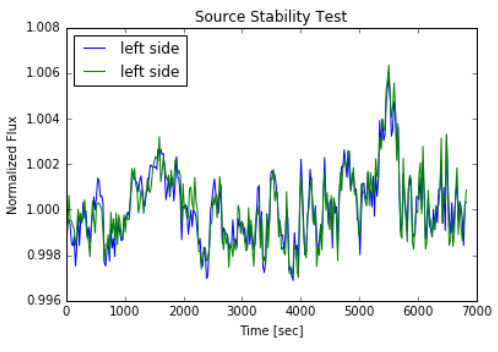
\includegraphics[width=0.5\textwidth]{stability2}
    \caption{Comparing time series from both sides}
    \end{centering}
\end{figure}

The right side deviates from the left side by about 10\%. 



\section{Different NIRCam Tests}
In the previous section, we discussed the general method of analyzing a test and gave example plots and curves. In this section we will provide the data analysis of actual tests as obtained by the methods described earlier. For each test, the extracted time series (for a and b detectors separately \& averaged), the averaged light curve with housing temperatures, linear best fit with ideal noise and measured noise vs. time plot will be provided. We average the light curves from two detectors because they are anti-correlated. 


\subsection{Test 1: WLP8SUB} 
\begin{figure}[H]
    \centering
    \begin{subfigure}{1}
        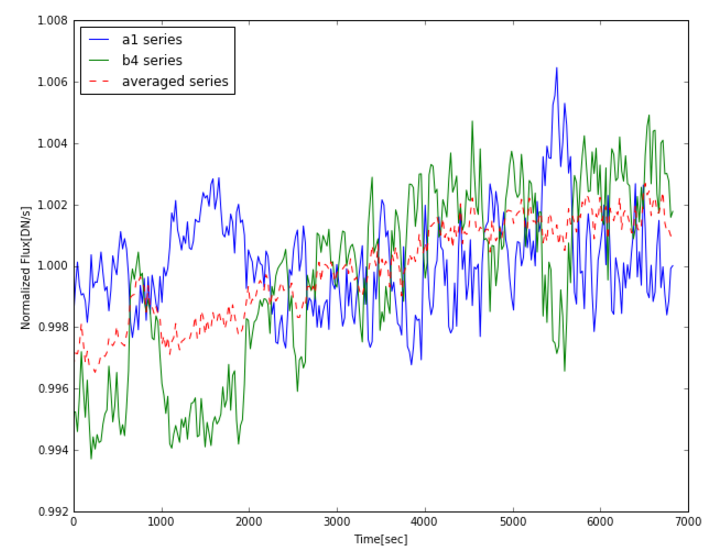
\includegraphics[scale=0.4]{ts_test1}
        \caption{Light curves of a1 series, b4 series and their average}
    \end{subfigure}

    \begin{subfigure}{2}
        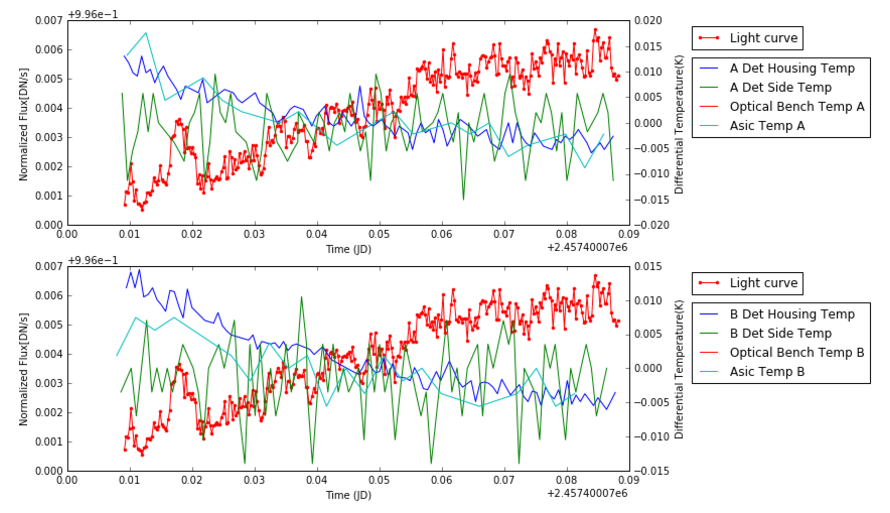
\includegraphics[scale=0.4]{temp_test1}
        \caption{The averaged light curve compared with detector temperatures}
    \end{subfigure}
   
    \begin{subfigure}{3}
        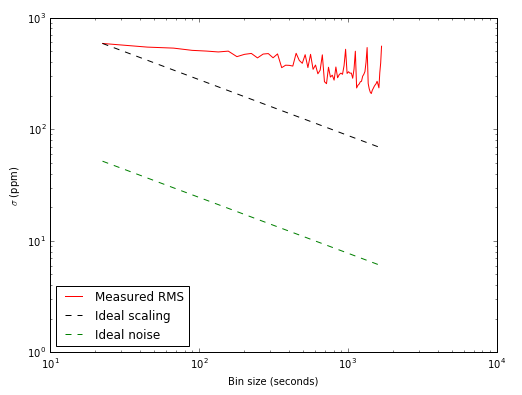
\includegraphics[scale=0.6]{rms_test1}
        \caption{RMS Vs. Bin size}
    \end{subfigure}
    \caption{Analysis of Test 1: WLP8SUB}
\end{figure}


\subsection{Test 2: WLP8SUB640} 
\begin{figure}[H]
    \centering
    \begin{subfigure}{1}
        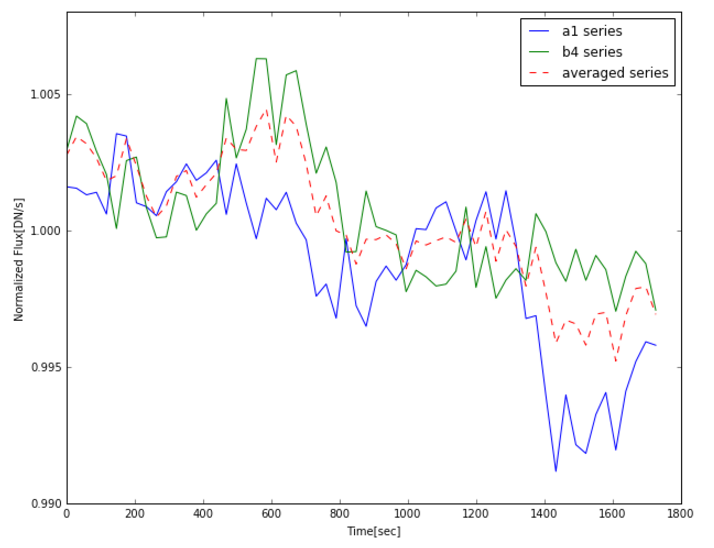
\includegraphics[scale=0.4]{ts_test2}
        \caption{Light curves of a1 series, b4 series and their average}
    \end{subfigure}

    \begin{subfigure}{2}
        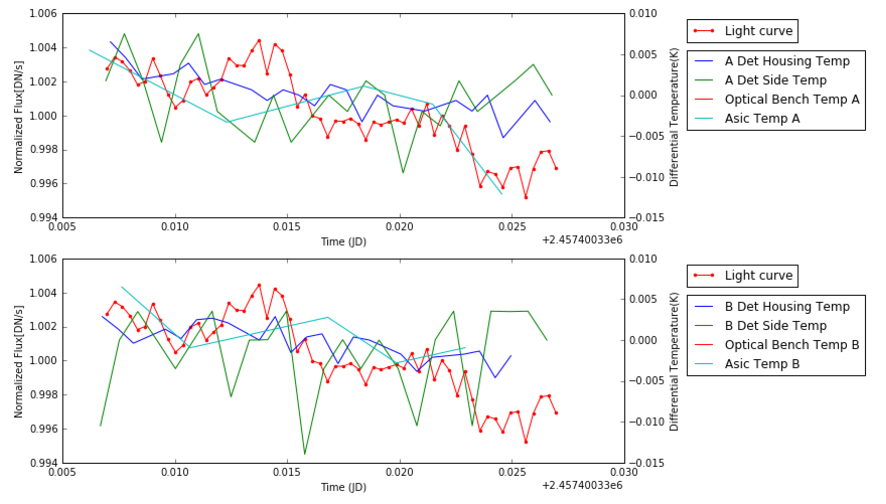
\includegraphics[scale=0.4]{temp_test2}
        \caption{The averaged light curve compared with detector temperatures}
    \end{subfigure}
   
    \begin{subfigure}{3}
        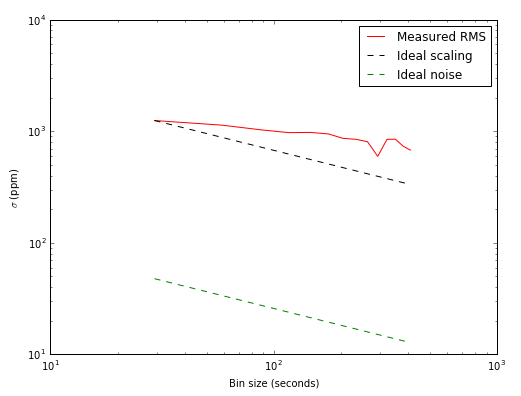
\includegraphics[scale=0.6]{rms_test2}
        \caption{RMS Vs. Bin size}
    \end{subfigure}
    \caption{Analysis of Test 2: WLP8SUB640}
\end{figure}


\subsection{Test 3: FULL0} 
\begin{figure}[H]
    \centering
    \begin{subfigure}{1}
        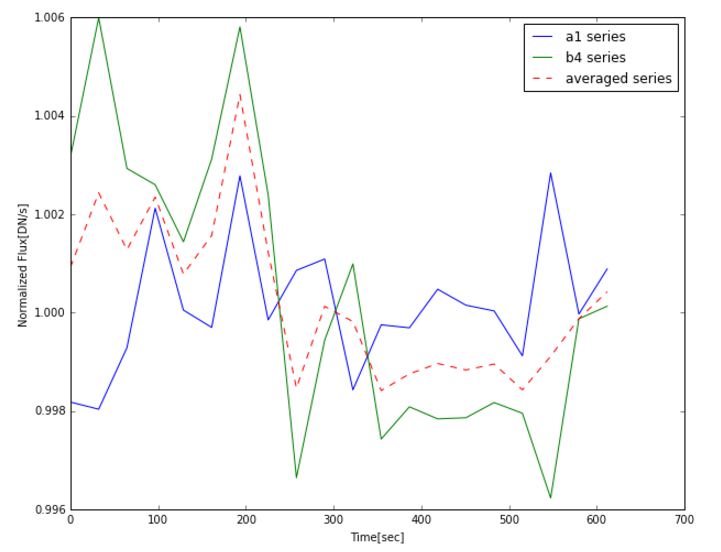
\includegraphics[scale=0.4]{ts_test3}
        \caption{Light curves of a1 series, b4 series and their average}
    \end{subfigure}

    \begin{subfigure}{2}
        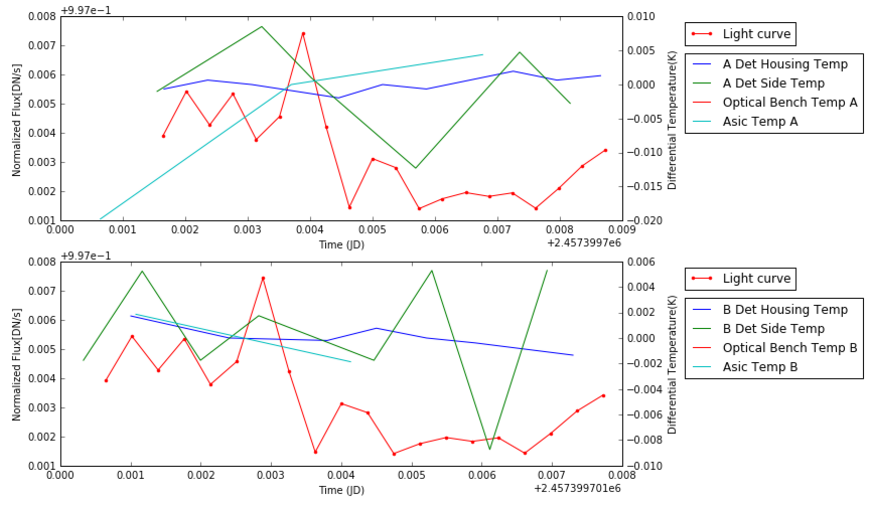
\includegraphics[scale=0.4]{temp_test3}
        \caption{The averaged light curve compared with detector temperatures}
    \end{subfigure}
   
    \begin{subfigure}{3}
        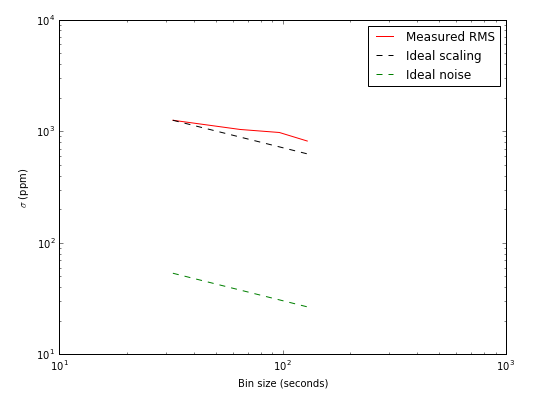
\includegraphics[scale=0.6]{rms_test3}
        \caption{RMS Vs. Bin size}
    \end{subfigure}
    \caption{Analysis of Test 3: FULL0}
\end{figure}


\subsection{Test 4: FULL1} 
\begin{figure}[H]
    \centering
    \begin{subfigure}{1}
        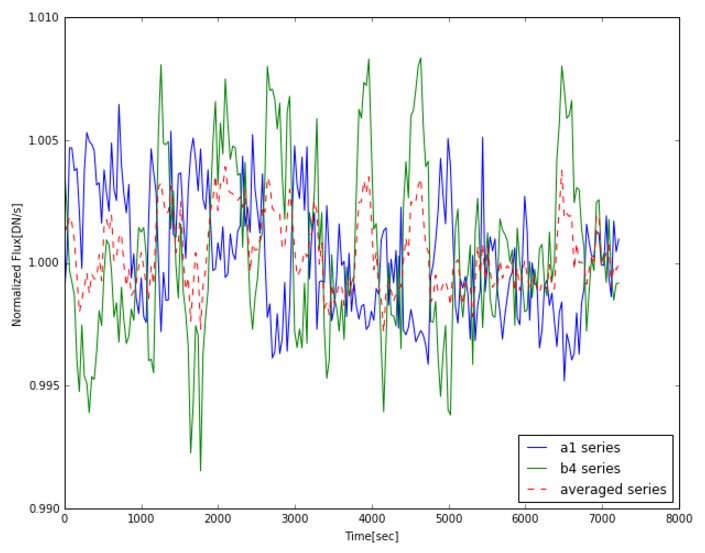
\includegraphics[scale=0.4]{ts_test4}
        \caption{Light curves of a1 series, b4 series and their average}
    \end{subfigure}

    \begin{subfigure}{2}
        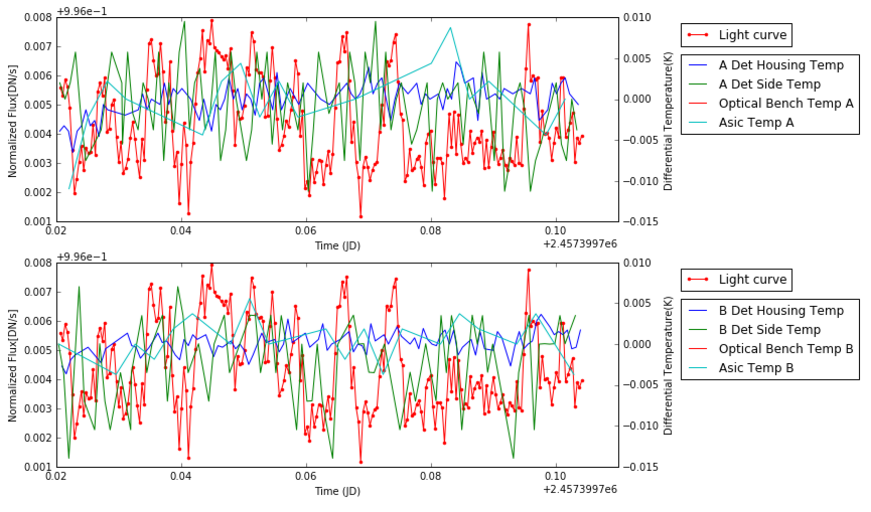
\includegraphics[scale=0.4]{temp_test4}
        \caption{The averaged light curve compared with detector temperatures}
    \end{subfigure}
   
    \begin{subfigure}{3}
        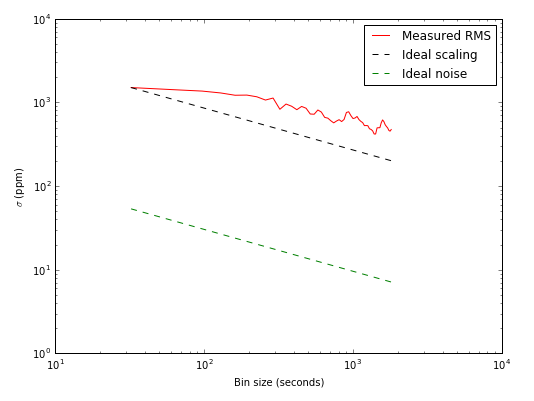
\includegraphics[scale=0.6]{rms_test4}
        \caption{RMS Vs. Bin size}
    \end{subfigure}
    \caption{Analysis of Test 4: FULL1}
\end{figure}


\subsection{Test 5: FULL2} 
\begin{figure}[H]
    \centering
    \begin{subfigure}{1}
        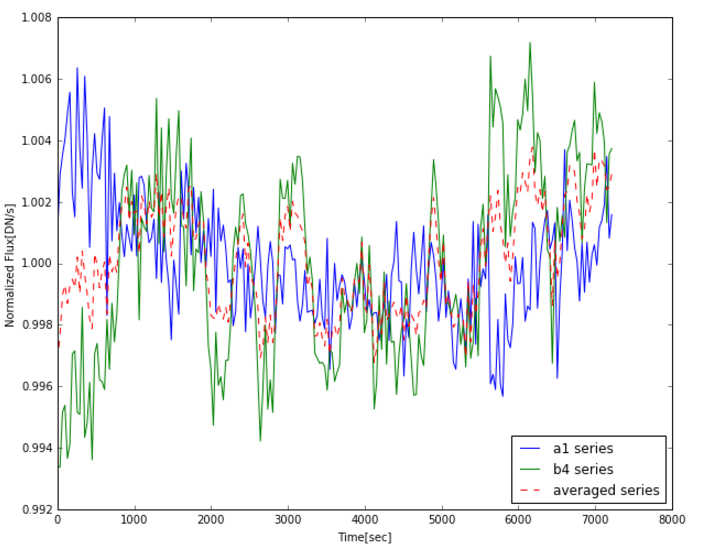
\includegraphics[scale=0.4]{ts_test5}
        \caption{Light curves of a1 series, b4 series and their average}
    \end{subfigure}

    \begin{subfigure}{2}
        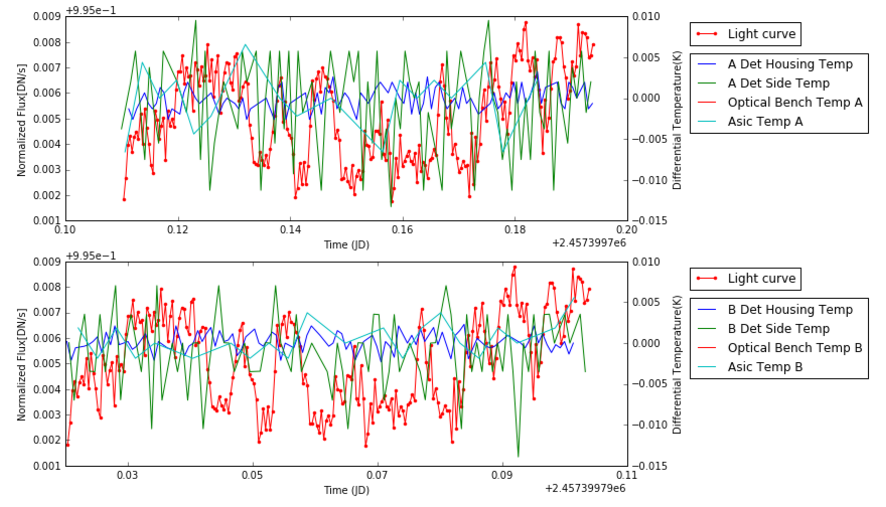
\includegraphics[scale=0.4]{temp_test5}
        \caption{The averaged light curve compared with detector temperatures}
    \end{subfigure}
   
    \begin{subfigure}{3}
        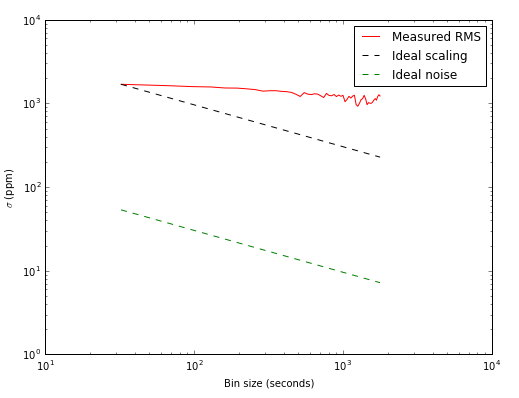
\includegraphics[scale=0.6]{rms_test5}
        \caption{RMS Vs. Bin size}
    \end{subfigure}
    \caption{Analysis of Test 5: FULL2}
\end{figure}


\subsection{Test 6: FULL3} 
\begin{figure}[H]
    \centering
    \begin{subfigure}{1}
        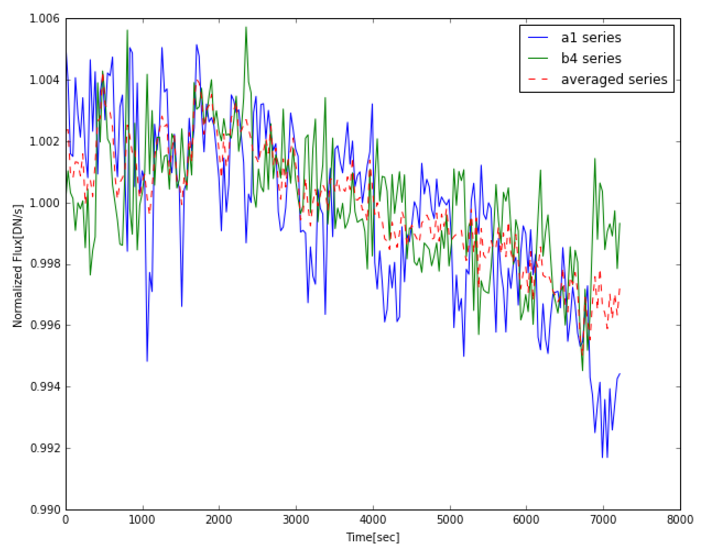
\includegraphics[scale=0.4]{ts_test6}
        \caption{Light curves of a1 series, b4 series and their average}
    \end{subfigure}

    \begin{subfigure}{2}
        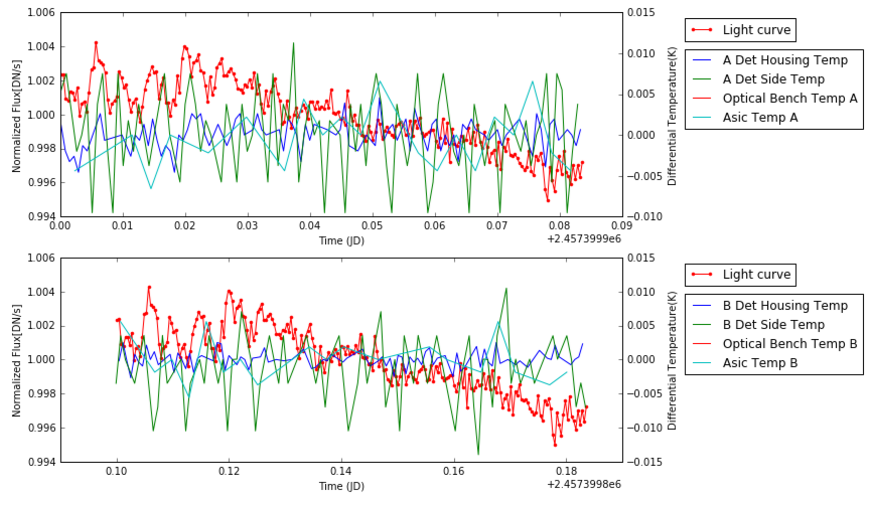
\includegraphics[scale=0.4]{temp_test6}
        \caption{The averaged light curve compared with detector temperatures}
    \end{subfigure}
   
    \begin{subfigure}{3}
        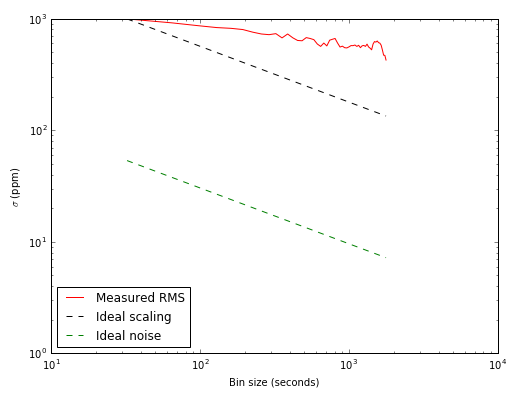
\includegraphics[scale=0.6]{rms_test6}
        \caption{RMS Vs. Bin size}
    \end{subfigure}
    \caption{Analysis of Test 6: FULL3}
\end{figure}


\subsection{Test 7: FULL4} 
\begin{figure}[H]
    \centering
    \begin{subfigure}{1}
        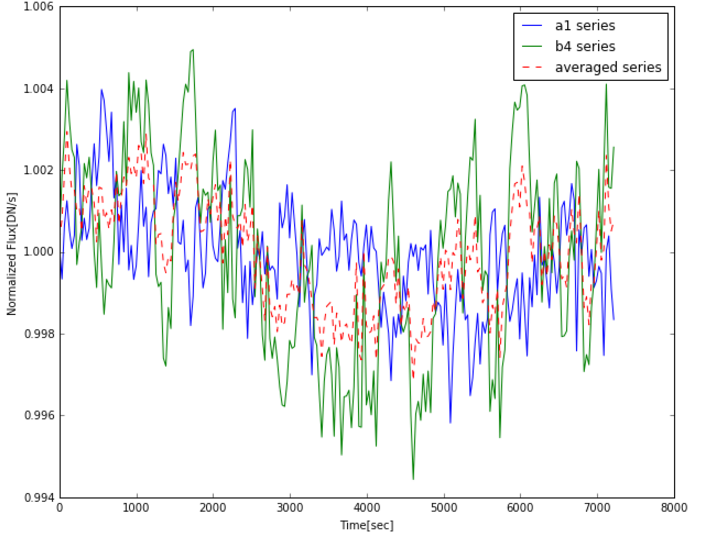
\includegraphics[scale=0.4]{ts_test7}
        \caption{Light curves of a1 series, b4 series and their average}
    \end{subfigure}

    \begin{subfigure}{2}
        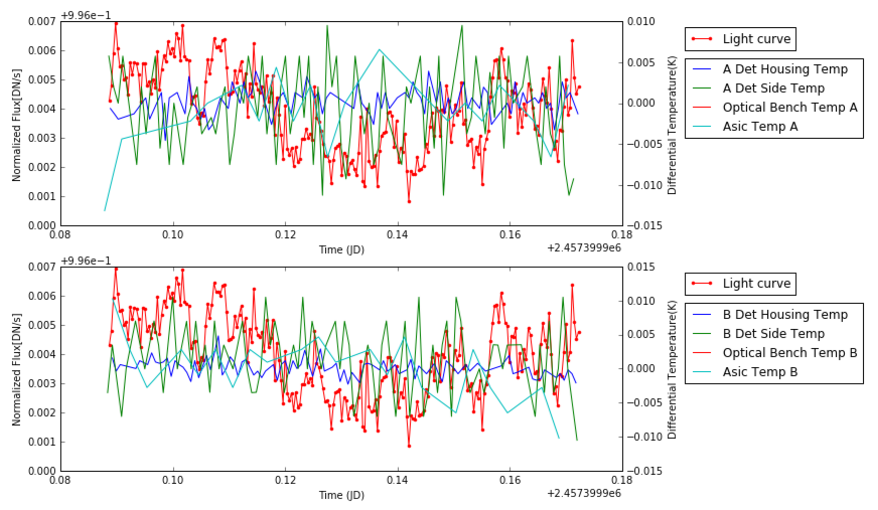
\includegraphics[scale=0.4]{temp_test7}
        \caption{The averaged light curve compared with detector temperatures}
    \end{subfigure}
   
    \begin{subfigure}{3}
        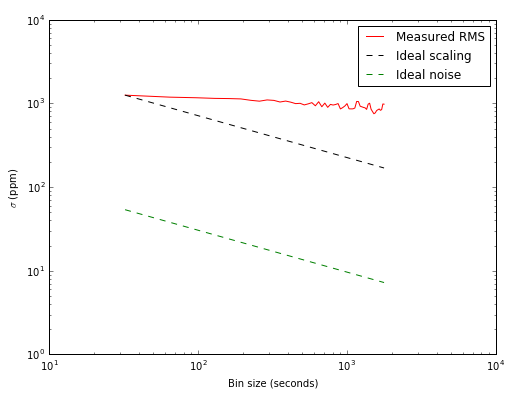
\includegraphics[scale=0.6]{rms_test7}
        \caption{RMS Vs. Bin size}
    \end{subfigure}
    \caption{Analysis of Test 7: FULL4}
\end{figure}


\subsection{Test 8: FULL5} 
\begin{figure}[H]
    \centering
    \begin{subfigure}{1}
        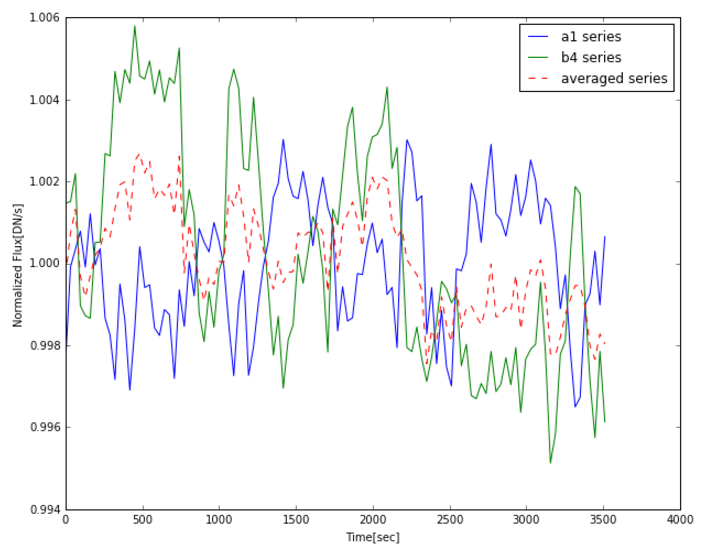
\includegraphics[scale=0.4]{ts_test8}
        \caption{Light curves of a1 series, b4 series and their average}
    \end{subfigure}

    \begin{subfigure}{2}
        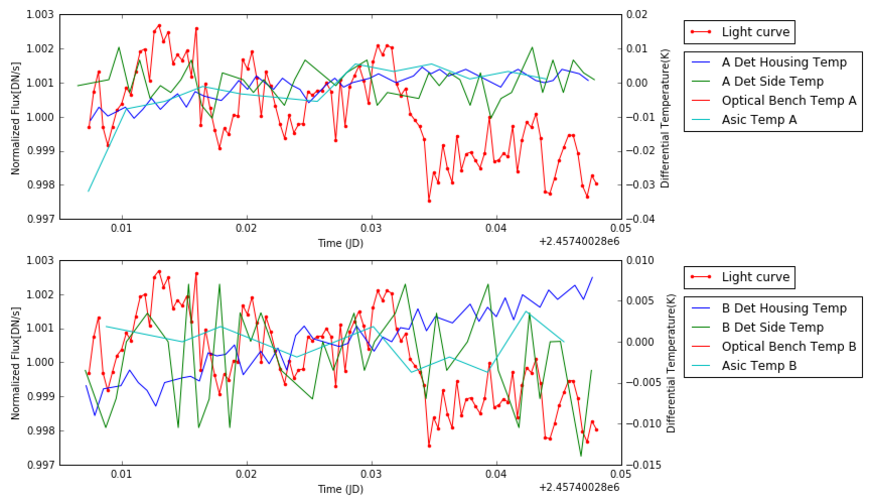
\includegraphics[scale=0.4]{temp_test8}
        \caption{The averaged light curve compared with detector temperatures}
    \end{subfigure}
   
    \begin{subfigure}{3}
        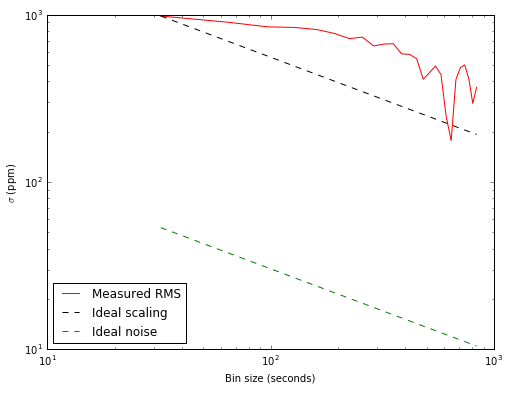
\includegraphics[scale=0.6]{rms_test8}
        \caption{RMS Vs. Bin size}
    \end{subfigure}
    \caption{Analysis of Test 8: FULL5}
\end{figure}


\subsection{Test 9: FULL6} 
\begin{figure}[H]
    \centering
    \begin{subfigure}{1}
        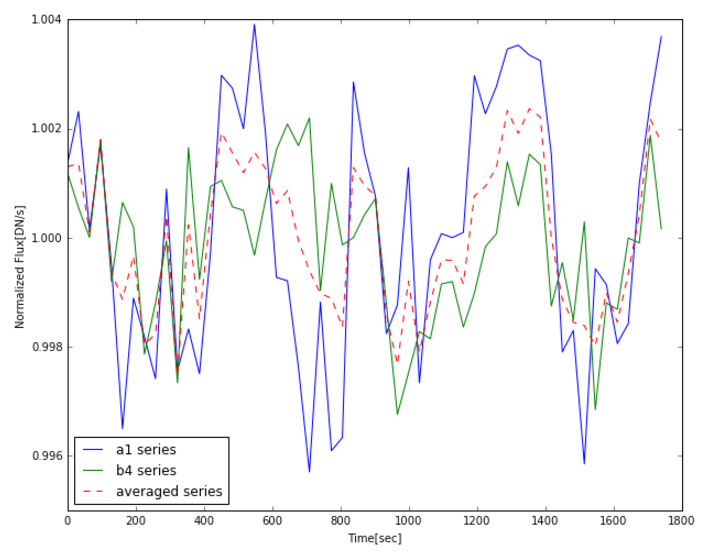
\includegraphics[scale=0.4]{ts_test9}
        \caption{Light curves of a1 series, b4 series and their average}
    \end{subfigure}

    \begin{subfigure}{2}
        \includegraphics[scale=0.4]{temp_test9}
        \caption{The averaged light curve compared with detector temperatures}
    \end{subfigure}
   
    \begin{subfigure}{3}
        \includegraphics[scale=0.6]{rms_test9}
        \caption{RMS Vs. Bin size}
    \end{subfigure}
    \caption{Analysis of Test 9: FULL6}
\end{figure}


\subsection{Test 10: FULL7} 
\begin{figure}[H]
    \centering
    \begin{subfigure}{1}
        \includegraphics[scale=0.4]{ts_test10}
        \caption{Light curves of a1 series, b4 series and their average}
    \end{subfigure}

    \begin{subfigure}{2}
        \includegraphics[scale=0.4]{temp_test10}
        \caption{The averaged light curve compared with detector temperatures}
    \end{subfigure}
   
    \begin{subfigure}{3}
        \includegraphics[scale=0.6]{rms_test10}
        \caption{RMS Vs. Bin size}
    \end{subfigure}
    \caption{Analysis of Test 10: FULL7}
\end{figure}


\subsection{Test 11: FULLQ} 
\begin{figure}[H]
    \centering
    \begin{subfigure}{1}
        \includegraphics[scale=0.4]{ts_test11}
        \caption{Light curves of a1 series, b4 series and their average}
    \end{subfigure}

    \begin{subfigure}{2}
        \includegraphics[scale=0.4]{temp_test11}
        \caption{The averaged light curve compared with detector temperatures}
    \end{subfigure}
   
    \begin{subfigure}{3}
        \includegraphics[scale=0.6]{rms_test11}
        \caption{RMS Vs. Bin size}
    \end{subfigure}
    \caption{Analysis of Test 11: FULLQ}
\end{figure}


\subsection{Test 12: FULL9} 
\begin{figure}[H]
    \centering
    \begin{subfigure}{1}
        \includegraphics[scale=0.4]{ts_test12}
        \caption{Light curves of a1 series, b4 series and their average}
    \end{subfigure}

    \begin{subfigure}{2}
        \includegraphics[scale=0.4]{temp_test12}
        \caption{The averaged light curve compared with detector temperatures}
    \end{subfigure}
   
    \begin{subfigure}{3}
        \includegraphics[scale=0.6]{rms_test12}
        \caption{RMS Vs. Bin size}
    \end{subfigure}
    \caption{Analysis of Test 12: FULL9}
\end{figure}


\subsection{Test 13: FULL10} 
\begin{figure}[H]
    \centering
    \begin{subfigure}{1}
        \includegraphics[scale=0.4]{ts_test13}
        \caption{Light curves of a1 series, b4 series and their average}
    \end{subfigure}

    \begin{subfigure}{2}
        \includegraphics[scale=0.4]{temp_test13}
        \caption{The averaged light curve compared with detector temperatures}
    \end{subfigure}
   
    \begin{subfigure}{3}
        \includegraphics[scale=0.6]{rms_test13}
        \caption{RMS Vs. Bin size}
    \end{subfigure}
    \caption{Analysis of Test 13: FULL10}
\end{figure}


\subsection{Test 14: FULL11} 
\begin{figure}[H]
    \centering
    \begin{subfigure}{1}
        \includegraphics[scale=0.4]{ts_test14}
        \caption{Light curves of a1 series, b4 series and their average}
    \end{subfigure}

    \begin{subfigure}{2}
        \includegraphics[scale=0.4]{temp_test14}
        \caption{The averaged light curve compared with detector temperatures}
    \end{subfigure}
   
    \begin{subfigure}{3}
        \includegraphics[scale=0.6]{rms_test14}
        \caption{RMS Vs. Bin size}
    \end{subfigure}
    \caption{Analysis of Test 14: FULL11}
\end{figure}


\subsection{Test 15: FULL12} 
\begin{figure}[H]
    \centering
    \begin{subfigure}{1}
        \includegraphics[scale=0.4]{ts_test15}
        \caption{Light curves of a1 series, b4 series and their average}
    \end{subfigure}

    \begin{subfigure}{2}
        \includegraphics[scale=0.4]{temp_test15}
        \caption{The averaged light curve compared with detector temperatures}
    \end{subfigure}
   
    \begin{subfigure}{3}
        \includegraphics[scale=0.6]{rms_test15}
        \caption{RMS Vs. Bin size}
    \end{subfigure}
    \caption{Analysis of Test 15: FULL12}
\end{figure}


\subsection{Test 16: FULL13} 
\begin{figure}[H]
    \centering
    \begin{subfigure}{1}
        \includegraphics[scale=0.4]{ts_test16}
        \caption{Light curves of a1 series, b4 series and their average}
    \end{subfigure}

    \begin{subfigure}{2}
        \includegraphics[scale=0.4]{temp_test16}
        \caption{The averaged light curve compared with detector temperatures}
    \end{subfigure}
   
    \begin{subfigure}{3}
        \includegraphics[scale=0.6]{rms_test16}
        \caption{RMS Vs. Bin size}
    \end{subfigure}
    \caption{Analysis of Test 16: FULL13}
\end{figure}


\subsection{Test 17: FULL14} 
\begin{figure}[H]
    \centering
    \begin{subfigure}{1}
        \includegraphics[scale=0.4]{ts_test17}
        \caption{Light curves of a1 series, b4 series and their average}
    \end{subfigure}

    \begin{subfigure}{2}
        \includegraphics[scale=0.4]{temp_test17}
        \caption{The averaged light curve compared with detector temperatures}
    \end{subfigure}
   
    \begin{subfigure}{3}
        \includegraphics[scale=0.6]{rms_test17}
        \caption{RMS Vs. Bin size}
    \end{subfigure}
    \caption{Analysis of Test 17: FULL14}
\end{figure}


\subsection{Test 18: CLRSUB1} 
\begin{figure}[H]
    \centering
    \begin{subfigure}{1}
        \includegraphics[scale=0.4]{ts_test18}
        \caption{Light curves of a1 series, b4 series and their average}
    \end{subfigure}

    \begin{subfigure}{2}
        \includegraphics[scale=0.4]{temp_test18}
        \caption{The averaged light curve compared with detector temperatures}
    \end{subfigure}
   
    \begin{subfigure}{3}
        \includegraphics[scale=0.6]{rms_test18}
        \caption{RMS Vs. Bin size}
    \end{subfigure}
    \caption{Analysis of Test 18: CLRSUB1}
\end{figure}


\subsection{Test 19: CLRSUB2} 
\begin{figure}[H]
    \centering
    \begin{subfigure}{1}
        \includegraphics[scale=0.4]{ts_test19}
        \caption{Light curves of a1 series, b4 series and their average}
    \end{subfigure}

    \begin{subfigure}{2}
        \includegraphics[scale=0.4]{temp_test19}
        \caption{The averaged light curve compared with detector temperatures}
    \end{subfigure}
   
    \begin{subfigure}{3}
        \includegraphics[scale=0.6]{rms_test19}
        \caption{RMS Vs. Bin size}
    \end{subfigure}
    \caption{Analysis of Test 19: CLRSUB2}
\end{figure}


\subsection{Test 20: CLRSUB3} 
\begin{figure}[H]
    \centering
    \begin{subfigure}{1}
        \includegraphics[scale=0.4]{ts_test20}
        \caption{Light curves of a1 series, b4 series and their average}
    \end{subfigure}

    \begin{subfigure}{2}
        \includegraphics[scale=0.4]{temp_test20}
        \caption{The averaged light curve compared with detector temperatures}
    \end{subfigure}
   
    \begin{subfigure}{3}
        \includegraphics[scale=0.6]{rms_test20}
        \caption{RMS Vs. Bin size}
    \end{subfigure}
    \caption{Analysis of Test 20: CLRSUB3}
\end{figure}


\subsection{Test 21: CLRSUB4} 
\begin{figure}[H]
    \centering
    \begin{subfigure}{1}
        \includegraphics[scale=0.4]{ts_test21}
        \caption{Light curves of a1 series, b4 series and their average}
    \end{subfigure}

    \begin{subfigure}{2}
        \includegraphics[scale=0.4]{temp_test21}
        \caption{The averaged light curve compared with detector temperatures}
    \end{subfigure}
   
    \begin{subfigure}{3}
        \includegraphics[scale=0.6]{rms_test21}
        \caption{RMS Vs. Bin size}
    \end{subfigure}
    \caption{Analysis of Test 21: CLRSUB4}
\end{figure}


\subsection{Test 22: CLRSUB5} 
\begin{figure}[H]
    \centering
    \begin{subfigure}{1}
        \includegraphics[scale=0.4]{ts_test22}
        \caption{Light curves of a1 series, b4 series and their average}
    \end{subfigure}

    \begin{subfigure}{2}
        \includegraphics[scale=0.4]{temp_test22}
        \caption{The averaged light curve compared with detector temperatures}
    \end{subfigure}
   
    \begin{subfigure}{3}
        \includegraphics[scale=0.6]{rms_test22}
        \caption{RMS Vs. Bin size}
    \end{subfigure}
    \caption{Analysis of Test 22: CLRSUB5}
\end{figure}


\subsection{Test 23: CLRSUB6} 
\begin{figure}[H]
    \centering
    \begin{subfigure}{1}
        \includegraphics[scale=0.4]{ts_test23}
        \caption{Light curves of a1 series, b4 series and their average}
    \end{subfigure}

    \begin{subfigure}{2}
        \includegraphics[scale=0.4]{temp_test23}
        \caption{The averaged light curve compared with detector temperatures}
    \end{subfigure}
   
    \begin{subfigure}{3}
        \includegraphics[scale=0.6]{rms_test23}
        \caption{RMS Vs. Bin size}
    \end{subfigure}
    \caption{Analysis of Test 23: CLRSUB6}
\end{figure}


\subsection{Test 24: WLP8A1B4} 
\begin{figure}[H]
    \centering
    \begin{subfigure}{1}
        \includegraphics[scale=0.4]{ts_test24}
        \caption{Light curves of a1 series, b4 series and their average}
    \end{subfigure}

    \begin{subfigure}{2}
        \includegraphics[scale=0.4]{temp_test24}
        \caption{The averaged light curve compared with detector temperatures}
    \end{subfigure}
   
    \begin{subfigure}{3}
        \includegraphics[scale=0.6]{rms_test24}
        \caption{RMS Vs. Bin size}
    \end{subfigure}
    \caption{Analysis of Test 24: WLP8A1B4}
\end{figure}


\subsection{Test 25: WLP8A2B3} 
\begin{figure}[H]
    \centering
    \begin{subfigure}{1}
        \includegraphics[scale=0.4]{ts_test25}
        \caption{Light curves of a1 series, b4 series and their average}
    \end{subfigure}

    \begin{subfigure}{2}
        \includegraphics[scale=0.4]{temp_test25}
        \caption{The averaged light curve compared with detector temperatures}
    \end{subfigure}
   
    \begin{subfigure}{3}
        \includegraphics[scale=0.6]{rms_test25}
        \caption{RMS Vs. Bin size}
    \end{subfigure}
    \caption{Analysis of Test 25: WLP8A2B3}
\end{figure}


\subsection{Test 26: WLP8A3B2} 
\begin{figure}[H]
    \centering
    \begin{subfigure}{1}
        \includegraphics[scale=0.4]{ts_test26}
        \caption{Light curves of a1 series, b4 series and their average}
    \end{subfigure}

    \begin{subfigure}{2}
        \includegraphics[scale=0.4]{temp_test26}
        \caption{The averaged light curve compared with detector temperatures}
    \end{subfigure}
   
    \begin{subfigure}{3}
        \includegraphics[scale=0.6]{rms_test26}
        \caption{RMS Vs. Bin size}
    \end{subfigure}
    \caption{Analysis of Test 26: WLP8A3B2}
\end{figure}



\section{Conclusion}
After analyzing the tests, we found that the best way to process the data involves the following methods: 1) Generating separate centers for each image 2) Doing a linear fitting to remove trend 3) Using Slope2 method for files with $NGROUP = 2$ 4) Using annular aperture function rather than median subtraction to subtract background \& 5) Using MMM tests, i.e. apply no correction method  

\bibliographystyle{aasjournal}

\end{document}
